\chapter{基于解的局部性的自适应优化方法}
在上一章中,本研究发现了LazyAsync的性能提升的相对大小和冗余计算的比例有关。
为了得到更好的性能提升,LazyAsync需要尽可能的避免冗余计算。
在本章中,从如何降低冗余计算比例这一问题出发,本研究最终实现了基于解的局部性这一自适应优化方法。
在这一方法指导的开启策略下,LazyAsync获得了相对最优的性能提升。

在本章中,本研究先是从单个顶点的角度出发分析了全局解和局部解的局部性关系有利于减少冗余计算。
然后通过实验对图计算过程中全体活跃点上全局解和局部解的关系进行了分析,发现了解的局部性这一规律。
从这一规律入手,通过在线统计的方法,本研究最终实现了基于解的局部性的自适应优化方法。
最后,本章在不同图算法和输入图的组合上对这种方法进行了评测,验证了它的性能提升效果。

\section{全局解和局部解如何影响冗余计算}

在分布式图计算中,由于副本点的存在,每个顶点上的全局解由多个局部解构成。
在把图计算迭代公式改写为差值累加的形式之后,图计算通过交换构成局部解的消息累加值然后进行计算来实现不同副本点上的全局解的一致。

当顶点上的全局解由多个局部解构成时,那么多个局部解都不等于全局解。
那么用这样的局部解进行的本地计算自然是冗余无效的。
当顶点上的全局解由单个局部解构成时,那么这个局部解就等于全局解。
用已经等于全局解的局部解进行本地计算自然是有效的。
同时由于其他副本上没有局部解,副本点就不记录为活跃点,也就不会产生本地计算。
这些副本会在数据一致性阶段收到消息,从而得到和全局解一致的视图。
也就是说就单个顶点而言,全局解由多个局部解构成时不利于开启LazyAsync,
全局解由单个局部解构成时有利于开启LazyAsync。


在图\ref{fig:useless_and_local}中,本研究再次以 SSSP 为例子直观的展示全局解和局部解如何影响冗余计算。
图\ref{fig:useless_and_local}中,左侧给出了一个全局解由多个局部解构成的例子,右侧给出了一个全局解由单个局部解构成的例子。
在左侧中,一个顶点在5台机器上分布着副本点,并且5台机器上分别存在着6,7,7,8,9这5个局部解。
根据SSSP中对局部解之间$\oplus$的定义:$a\oplus b=std::min(a,b)$,全局解为6。
所以只有一个局部解等于全局解,在机器1,2,3,4上的局部解都不等于全局解。
如果此时对这5个副本点使用LazyAsync,那么机器1,2,3,4上的副本点所进行的本地计算都是无效而冗余的。
在右侧中,同样是一个顶点在5台机器上分布着副本点,但是只在机器2上存在局部解,此时机器2上的局部解就是全局解。
如果此时对这5个副本使用LazyAsync,那么机器0,1,3,4上的副本由于没有收到消息不被激活,所以不产生本地计算。
机器2上的副本其局部解就等于全局解,所以机器2上所进行的本地计算是有效的。
在数据一致性阶段,机器0,1,3,4上的副本会通过消息交换得到和机器2上的副本同样的全局视图。



\begin{figure}[!htbp]
\centering
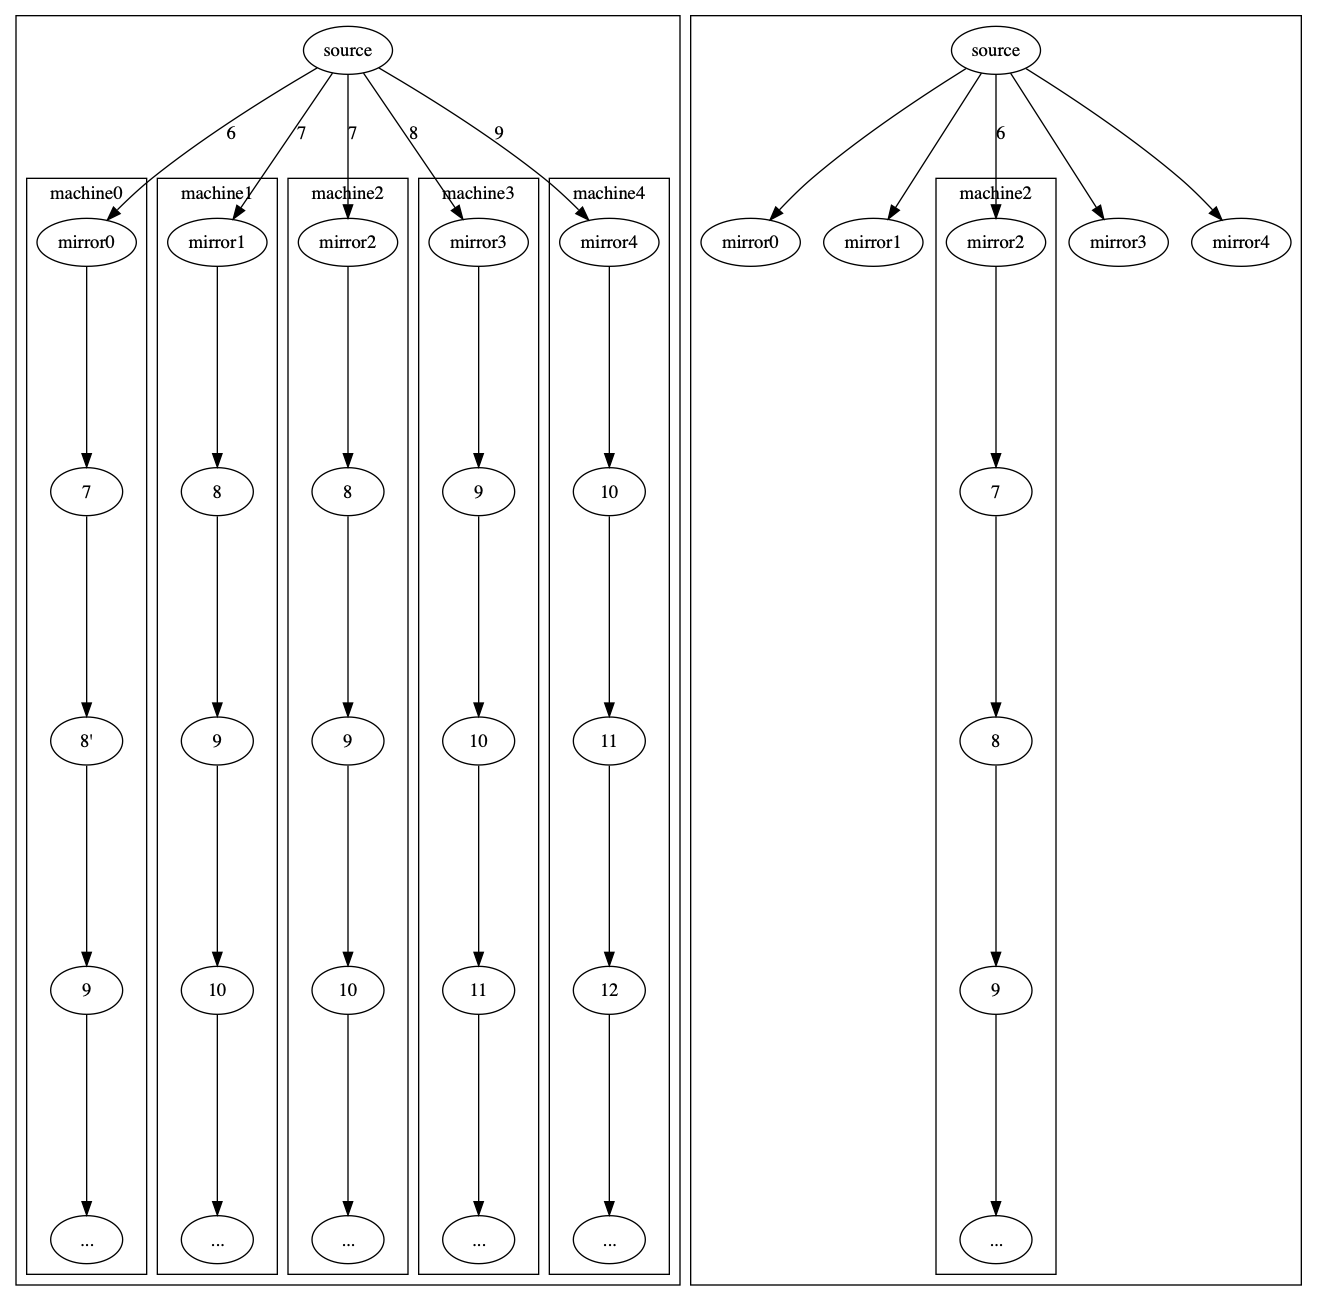
\includegraphics[width=0.8\textwidth]{useless_and_local}
\bicaption{解的局部性如何影响冗余计算}{How the locality of the solution affects redundant calculations}
\label{fig:useless_and_local}
\end{figure}


通过上边的例子可以看到,全局解由单个局部解构成时有利于开启lazy data coherency 。
分布式图计算框架把单个顶点划分为多个副本点。
在LazyAsync中,每次迭代时,顶点的全局解也就由多个副本点上的局部解构成。
从单个顶点的角度而言,
如果顶点的全局解由多个局部解构成,然后此时在各个局部解所在的副本点上进行LazyAsync,也就是在本地计算中进行额外的多轮迭代,
由于副本点上都是不准确的局部解,因而此时所进行的本地计算都是在不准确的结果上进行的,所以最终本地计算中更多是冗余计算。
相反,如果顶点的全局解只由某个局部解构成,那么在局部解所在的副本点上开启LazyAsync,
由于局部解就等于全局解,所以此时相当于在全局同步之后进行的迭代,那么此时所进行的本地计算中冗余计算的比例就较低。
也就是说,从单个顶点而言,当全局解只由某个局部解构成时,本地计算中冗余计算比例较低,有利于开启LazyAsync,
当全局解由多个局部解构成时,本地计算中冗余计算比例较高,不利于开启LazyAsync。

% 在图计算的每次迭代过程中有很多活跃点,这些活跃点中既有全局解由单个局部解构成的,也有全局解由多个局部解构成的。
在图计算过程中的任何时刻,全局解由单个局部解构成和由多个局部解构成的情况都是同时存在的。
如果大部分活跃点的全局解只由单个局部解构成,那么此时开启lazy data coherency 能够减少冗余计算,最终得到较好的性能提升。
% 但是如果大多数顶点的全局解都只由当局部解构成,那么此时显然是开启延迟数据一致性的良好时机。
对于这种情况,本研究称之为解的局部性。
% 这种情况本研究称之为解的局部性。

\section{全局解和局部解的关系中的局部性规律}
为了研究图计算过程中解的局部性的变化规律,本研究需要保存每次迭代过程中的局部解,然后对其进行观察。

在图计算过程中,局部解由本地的消息累加和构成。
这些消息累加和被包含在消息中然后在集群结点之间进行交换。
消息交换在图计算中起着重要作用,消息中的消息累加和承载了下一轮迭代有哪些活跃点以及这些活跃点收到的消息这些重要信息。
当消息为空时,系统中没有活跃点,图计算也就收敛结束了。

在m2m方式的消息交换中,系统通过三个阶段完成副本点之间的局部解的交换从而实现数据一致。
第一个阶段,所有的副本点向 master 点发送自己的消息累加和。
master 点收到所有副本点上的消息累加和之后按照事先定义的$\oplus$操作符对这些消息累加得到全局消息累加和。
此时进入第二个阶段,master 点向所有副本点发送全局消息累加和。
此时所有的副本点都得到了一份原有的本地消息和全局消息累加和。
由于全局消息累加和中存在着重复的本地消息,所以消息交换还需要第三个阶段,
每个副本点要在全局消息累加和中减去自己的本地消息。
最终经历这三个阶段,每个副本点都得到了相同的消息累加和从而得到相同的全局视图。


可以看到局部解直接体现为副本点的本地消息累加和。
但是图计算过程中并不关心副本点上的消息累加和之间的数量和相对数值,只关心最终的全局消息累加和。
消息交换完成得到全局消息累加和之后,代表着局部解的本地消息累加和就会被清空。
所以,为了记录局部解和全局解从而分析它们的规律,本研究需要给 vertex data 添加两个数据结构。
一个是$std::map<int,T> data\_at\_iter$用于记录第$i$次迭代时顶点的全局解。
一个是$std:map<int, std::vector<message\_type>> local\_sum$用于记录第$i$次迭代时
顶点收到的多个消息累加和。

在顶点进行全局的 apply 操作时,系统可以在顶点上记录下全局解。
为了记录消息累加和则需要在两个地方添加代码。
第一处是master点发送自己的本地消息累加和,由于不通过网络交换消息,这里可以直接写入。
第二处是为了记录mirror点向master点通过网络发送的本地消息累加和,需要在收消息的地方添加代码。
通过以上两个地方添加记录消息累加和的代码,保证了对局部解的记录是不重不漏的。 
需要说明的是,局部解的数量有可能少于副本点的数量。
因为那些不被激活的副本点是不会向 master 发送包含本地消息累加和的消息的。


图\ref{fig:local_sssp}给出了一个具体的顶点上记录到的全局解和消息累加和的例子。
图中第一列是顶点id,第二列是最终解,第三列是迭代解,第四列是副本点的数量,接下来是顶点上收到的多个消息累加和,
最后一列是顶点上一轮的迭代解。
以图中3629703号顶点为例,可以看到这个顶点有20个副本,全局解是6,由15个局部解构成,并且其中7个局部解都不等于全局解。
在这样的顶点上使用LazyAsync显然会造成一定数量的冗余计算。
而以图中411911号顶点为例,可以看到这个顶点也有20个副本,全局解是7,但是只由一个局部解构成。
那么像这样的顶点显然是存在着解的局部性的,使用LazyAsync不太容易造成冗余计算。


\begin{figure}[H]
  \centering
  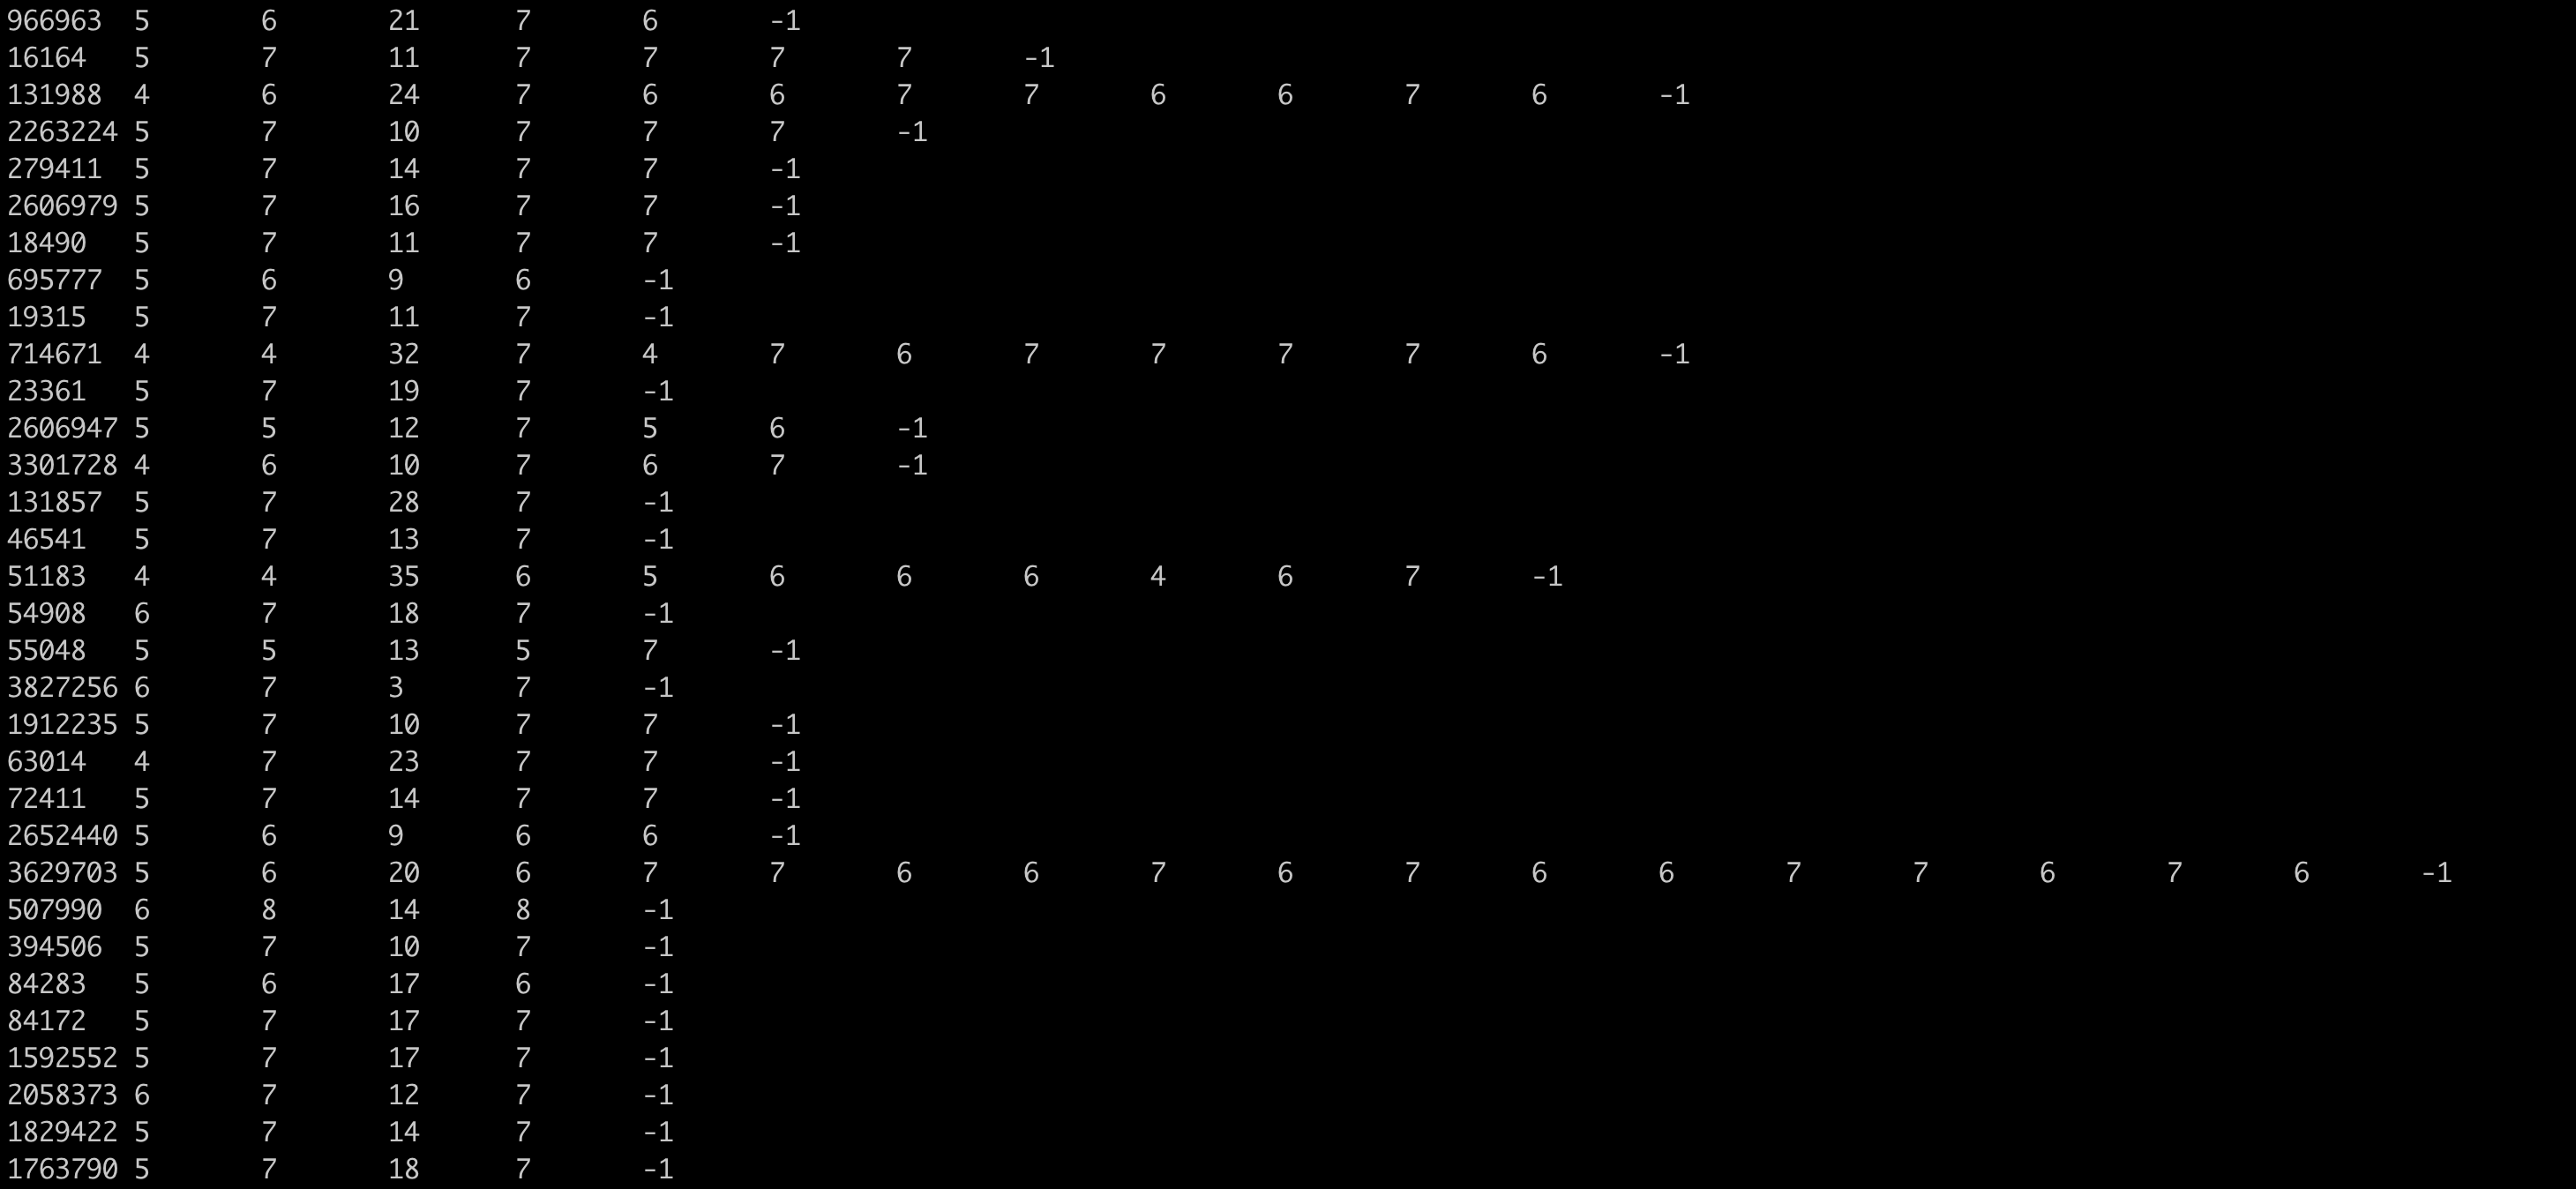
\includegraphics[width=0.8\textwidth]{local_sssp}
  \bicaption{局部解示意图}{Local solution diagram}
  \label{fig:local_sssp}
\end{figure}
%用mapreduce进行统计
通过记录具体的本地消息累加和,本研究可以观察在迭代过程中解的局部性的变化规律。
即图计算的迭代过程中,有多少顶点上的全局解是由单个局部解构成的,这样的顶点是否占多数。
图计算完成之后,运行时记录的全局解和局部解这些信息保存在了 graph 中。 
利用 PowerGraph 提供的 map-reduce 接口,本研究可以通过 graph 上记录的数据具体统计每一轮迭代中
全局解由多个和单个局部解构成的顶点的数量。

%统计结果


通过在计算引擎中添加代码和使用map-reduce接口进行统计,本研究在SSSP, 
Connected Component(CC),
PageRank 这3种常用的图算法和8个典型的图上进行实验对解的局部性规律进行了统计。
8个图数据集的元数据如表\ref{tab:experimental_data_set}所示,它们包含3个不同类型,下载自
Stanford Large Network Dataset Collection\cite{SNAP}、
the Laboratory for Web Algorithmic \cite{LAW}
和 the DIMACS shortest paths challenge\cite{DIMACS}。


\begin{table}[H]
  \centering
  \bicaption{实验数据集}{Experimental Data Set }
  \label{tab:experimental_data_set}
    \begin{tabular}{ccccccc}
     \toprule[1.5pt]
     & \textbf{Graph} & \textbf{\#V} & \textbf{\#E} & \textbf{E/V} & \textbf{$\lambda$} } \\
     \midrule[1pt]
     \multirow{2}{*}{web} & UK-2005 & 40M & 936M & 23.73 & 3.51  \\
                                         & web-Google & 0.9M & 5.1M & 5.83 & 2.47 \\
     \cmidrule(lr){1-6}
      \multirow{2}{*}{road} & road-USA-net & 24M & 58M & 2.44 & 2.14 \\
                                          & roadNet-CA & 2M & 5.5M & 2.82 & 2.09 \\
      \cmidrule(lr){1-6}
      \multirow{4}{*}{social} & twitter & 61.58M & 1468M & 23.85 & 5.52 \\
                                          & soc-LiveJournal & 4.84M & 68.9M & 14.23 & 4.96 \\
                                          & enwiki & 4.2M & 101.36M & 24.09M & 7.22 \\
                                          & com-youtube & 1.1M & 6M & 5.27M & 2.70 \\
     \bottomrule[1.5pt]
    \end{tabular}
\end{table}

实验结果如图\ref{fig:percent-sssp},\ref{fig:percent-cc},\ref{fig:percent-pg}所示。
图中分别给出了 SSSP,CC,PageRank 算法在 
web-Google, roadNet-CA,com-youtube
%USA-road, soc-LiveJournal, enwiki, uk-2005, twitter 
等8个大图上关于解的局部性规律的统计结果。
图中每个子图的横坐标轴代表了图计算过程的迭代轮次,
左侧纵坐标轴代表每次迭代的总的活跃点和由多个局部解构成全局解的活跃点的数量,
右侧纵坐标轴代表每次迭代的活跃点中具有局部性规律的活跃点的比例。
活跃点的局部性规律指的是它的全局解只由单个局部解构成。


\begin{figure}[H]
	\centering
  \captionsetup{justification=centering}
  \bisubcaptionbox{ Google 图上的统计结果\label{fig:percent-sssp-google}
}{Statistical results on the Google graph}
{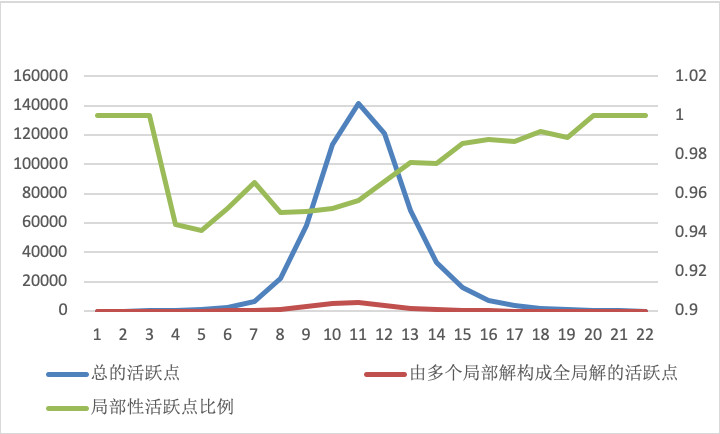
\includegraphics[height=3.8cm,width=0.4\textwidth]{percent-sssp-google.png}}
\hspace{4em}
\bisubcaptionbox{ CA-road 图上的统计结果\label{fig:percent-sssp-ca}
}{Statistical results on the CA-road graph}
{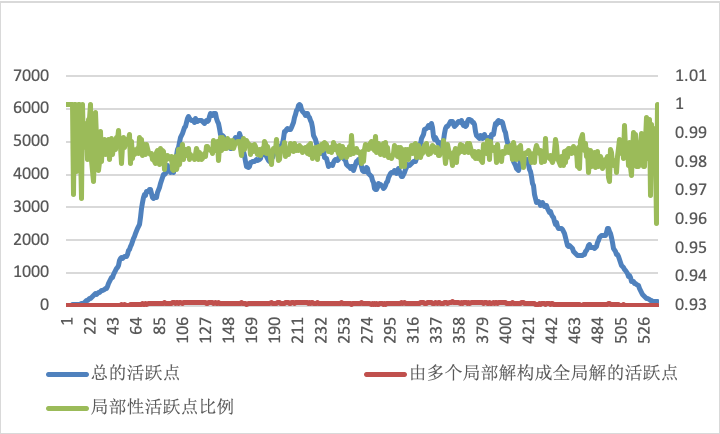
\includegraphics[height=3.8cm,width=0.4\textwidth]{percent-sssp-ca.png}}
\hspace{4em}
\bisubcaptionbox{ youtube 图上的统计结果\label{fig:percent-sssp-youtube}
}{Statistical results on the youtube graph}
{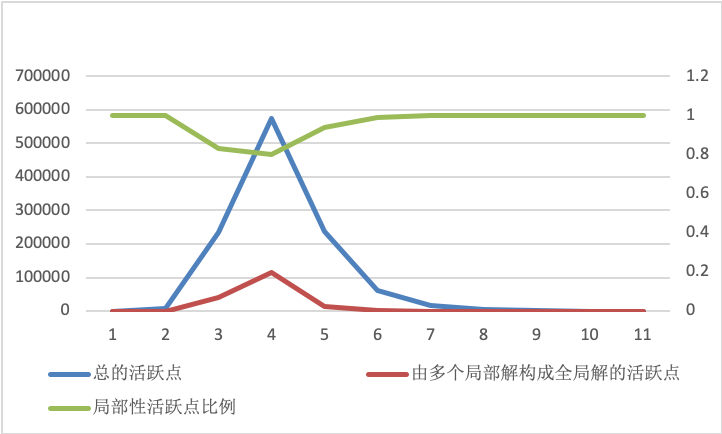
\includegraphics[height=3.8cm,width=0.4\textwidth]{percent-sssp-youtube.png}}
\hspace{4em}
\bisubcaptionbox{ USA-road 图上的统计结果\label{fig:percent-sssp-usa}
}{Statistical results on the USA-road graph}
{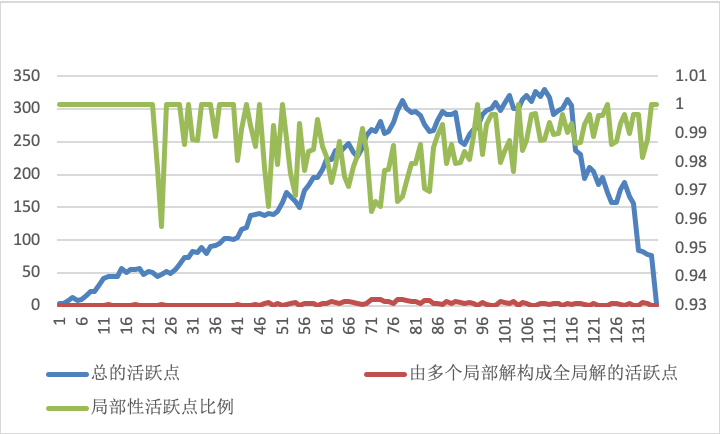
\includegraphics[height=3.8cm,width=0.4\textwidth]{percent-sssp-usa.png}}
\hspace{4em}
\bisubcaptionbox{ soc-Live 图上的统计结果\label{fig:percent-sssp-soc}
}{Statistical results on the soc-Live graph}
{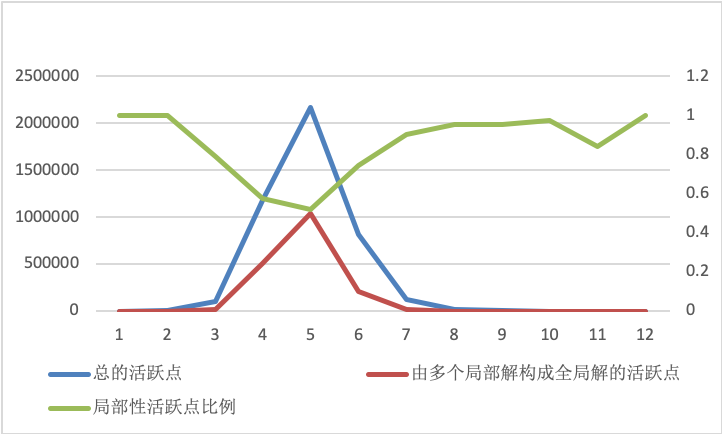
\includegraphics[height=3.8cm,width=0.4\textwidth]{percent-sssp-soc.png}}
\hspace{4em}
\bisubcaptionbox{ enwiki 图上的统计结果\label{fig:percent-sssp-enwiki}
}{Statistical results on the enwiki graph}
{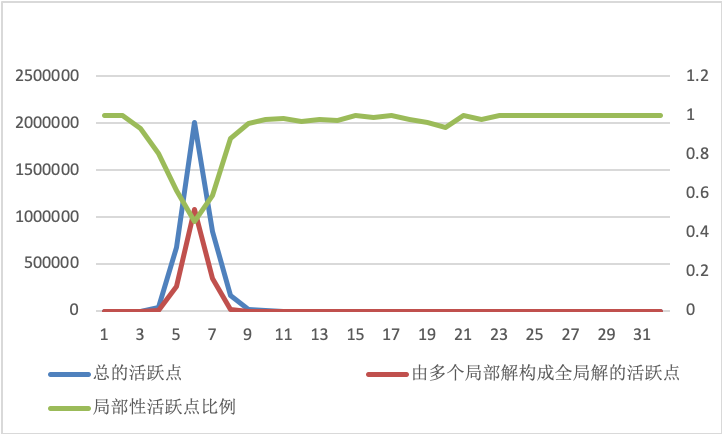
\includegraphics[height=3.8cm,width=0.4\textwidth]{percent-sssp-enwiki.png}}
\hspace{4em}
\bisubcaptionbox{ uk-2005 图上的统计结果\label{fig:percent-sssp-uk}
}{Statistical results on the uk-2005 graph}
{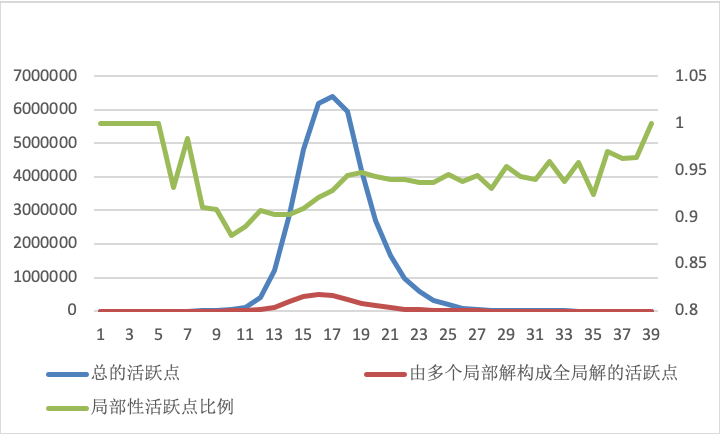
\includegraphics[height=3.8cm,width=0.4\textwidth]{percent-sssp-uk.png}}
\hspace{4em}
\bisubcaptionbox{ twitter 图上的统计结果\label{fig:percent-sssp-ntw}
}{Statistical results on the twitter graph}
{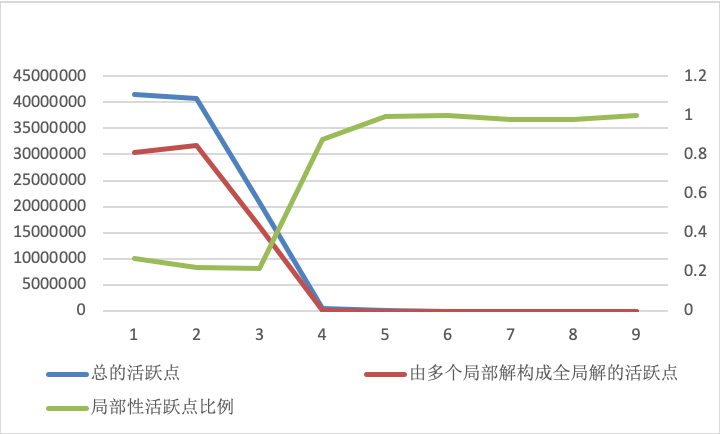
\includegraphics[height=3.8cm,width=0.4\textwidth]{percent-sssp-ntw.png}}
\hspace{4em}

  \bicaption{SSSP 算法在不同图上解的局部性的规律统计结果}{Statistical results for the regularity of local solutions of the SSSP algorithm on different graphs.
}
	\label{fig:percent-sssp}
\end{figure}




\begin{figure}[H]
	\centering
  \captionsetup{justification=centering}
  \bisubcaptionbox{ Google 图上的统计结果\label{fig:percent-cc-google}
}{Statistical results on the Google graph}
{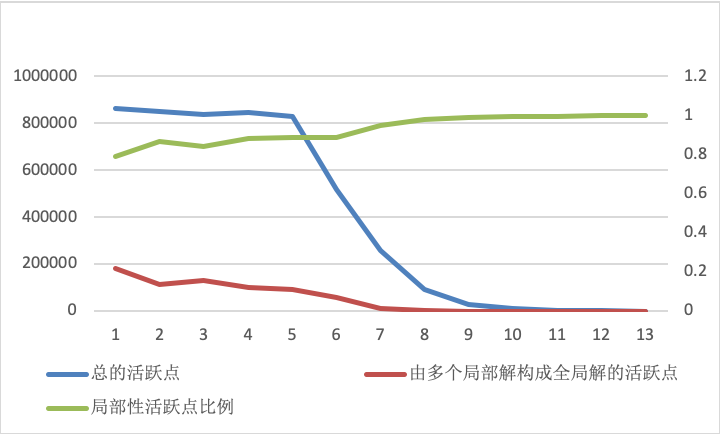
\includegraphics[height=3.8cm,width=0.4\textwidth]{percent-cc-google.png}}
\hspace{4em}
\bisubcaptionbox{ CA-road 图上的统计结果\label{fig:percent-cc-ca}
}{Statistical results on the CA-road graph}
{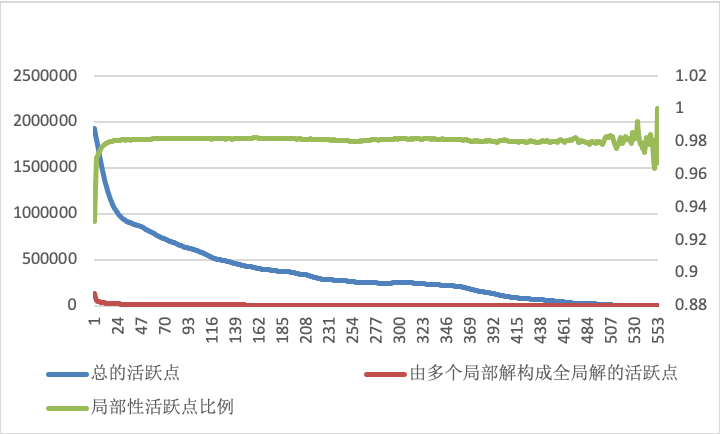
\includegraphics[height=3.8cm,width=0.4\textwidth]{percent-cc-ca.png}}
\hspace{4em}
\bisubcaptionbox{ youtube 图上的统计结果\label{fig:percent-cc-youtube}
}{Statistical results on the youtube graph}
{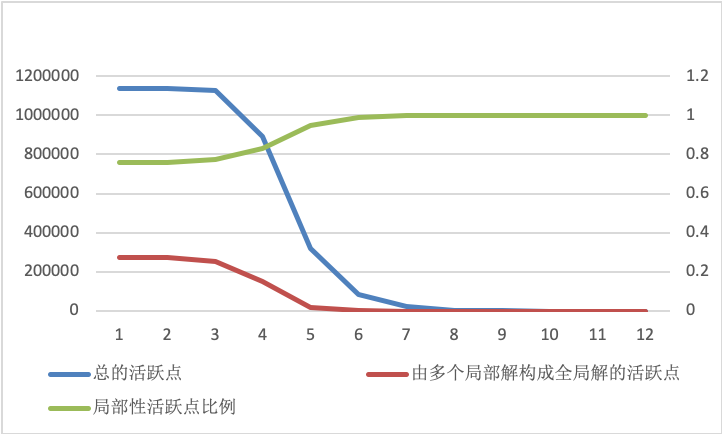
\includegraphics[height=3.8cm,width=0.4\textwidth]{percent-cc-youtube.png}}
\hspace{4em}
\bisubcaptionbox{ USA-road 图上的统计结果\label{fig:percent-cc-usa}
}{Statistical results on the USA-road graph}
{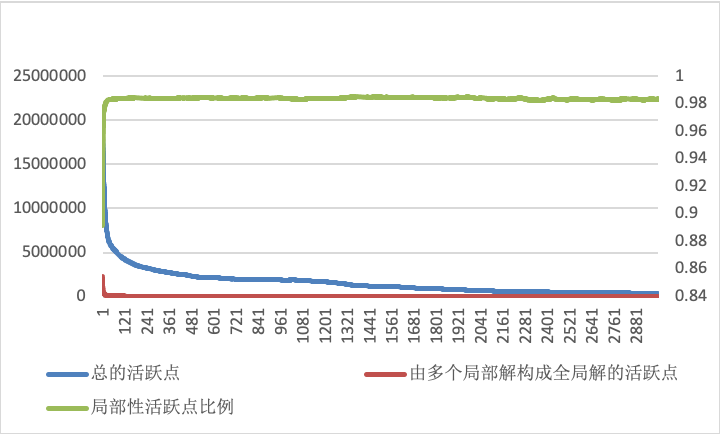
\includegraphics[height=3.8cm,width=0.4\textwidth]{percent-cc-usa.png}}
\hspace{4em}
\bisubcaptionbox{ soc-Live 图上的统计结果\label{fig:percent-cc-soc}
}{Statistical results on the soc-Live graph}
{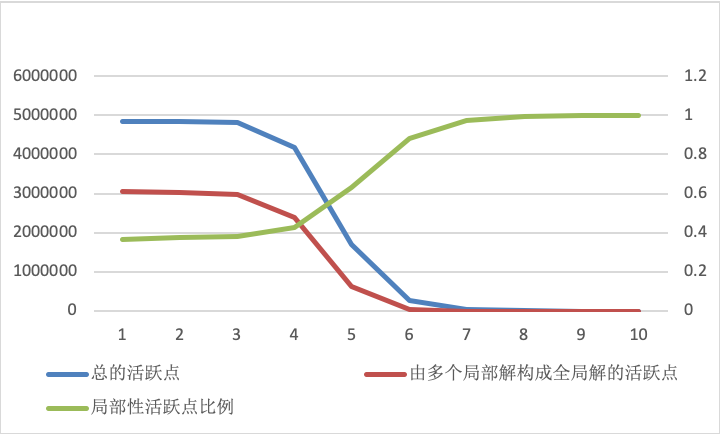
\includegraphics[height=3.8cm,width=0.4\textwidth]{percent-cc-soc.png}}
\hspace{4em}
\bisubcaptionbox{ enwiki 图上的统计结果\label{fig:percent-cc-enwiki}
}{Statistical results on the enwiki graph}
{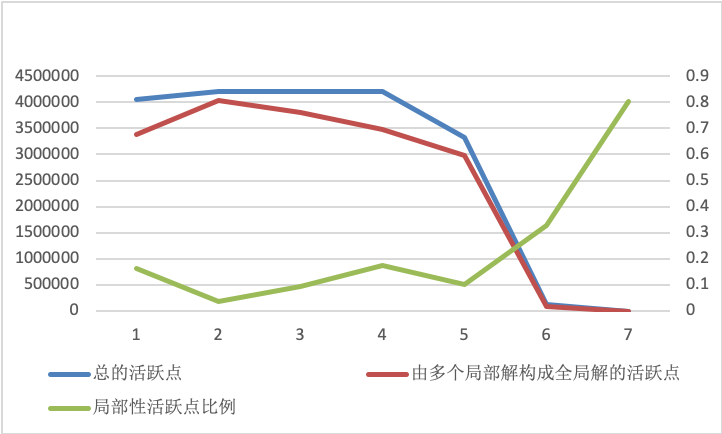
\includegraphics[height=3.8cm,width=0.4\textwidth]{percent-cc-enwiki.png}}
\hspace{4em}
\bisubcaptionbox{ uk-2005 图上的统计结果\label{fig:percent-cc-uk}
}{Statistical results on the uk-2005 graph}
{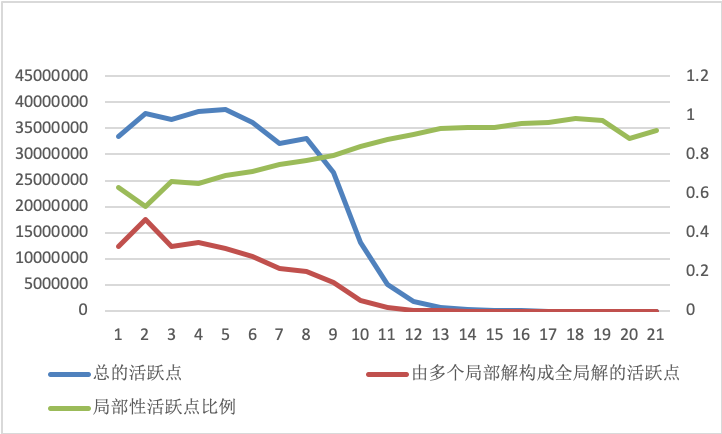
\includegraphics[height=3.8cm,width=0.4\textwidth]{percent-cc-uk.png}}
\hspace{4em}
\bisubcaptionbox{ twitter 图上的统计结果\label{fig:percent-cc-ntw}
}{Statistical results on the twitter graph}
{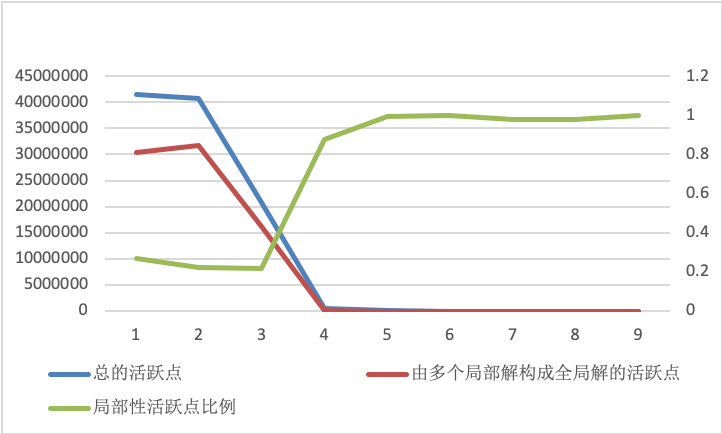
\includegraphics[height=3.8cm,width=0.4\textwidth]{percent-cc-ntw.png}}
\hspace{4em}

  \bicaption{CC 算法在不同图上解的局部性的规律统计结果}{Statistical results for the regularity of local solutions of the CC algorithm on different graphs.
}
	\label{fig:percent-cc}
\end{figure}

\begin{figure}[H]
	\centering
  \captionsetup{justification=centering}
  \bisubcaptionbox{ Google 图上的统计结果\label{fig:percent-pg-google}
}{Statistical results on the Google graph}
{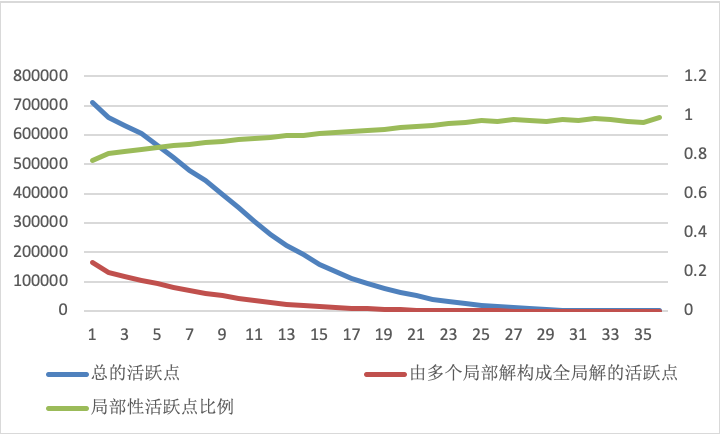
\includegraphics[height=3.8cm,width=0.4\textwidth]{percent-pg-google.png}}
\hspace{4em}
\bisubcaptionbox{ CA-road 图上的统计结果\label{fig:percent-pg-ca}
}{Statistical results on the CA-road graph}
{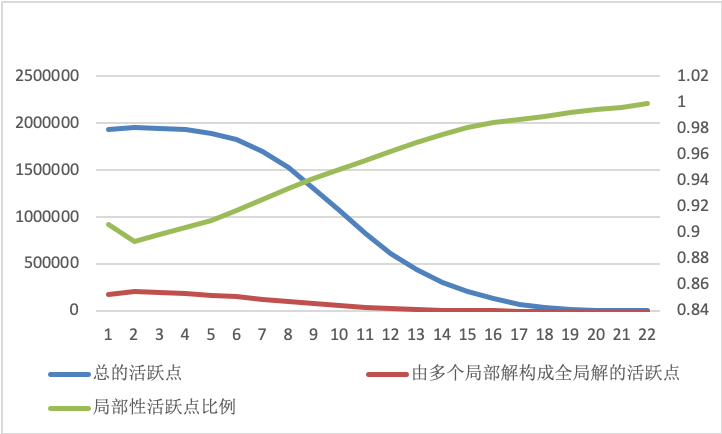
\includegraphics[height=3.8cm,width=0.4\textwidth]{percent-pg-ca.png}}
\hspace{4em}
\bisubcaptionbox{ youtube 图上的统计结果\label{fig:percent-pg-youtube}
}{Statistical results on the youtube graph}
{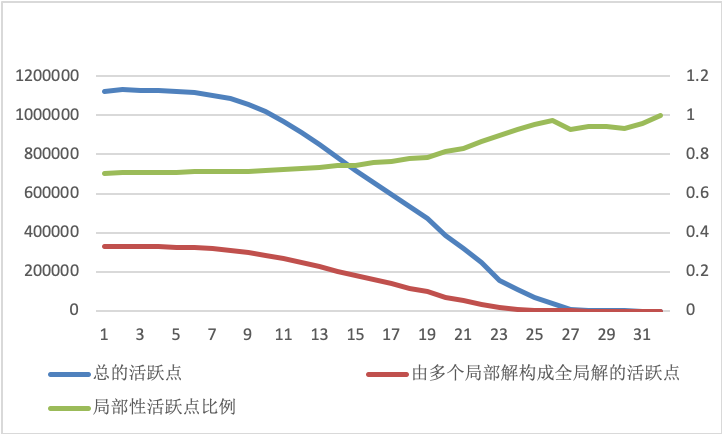
\includegraphics[height=3.8cm,width=0.4\textwidth]{percent-pg-youtube.png}}
\hspace{4em}
\bisubcaptionbox{ USA-road 图上的统计结果\label{fig:percent-pg-usa}
}{Statistical results on the USA-road graph}
{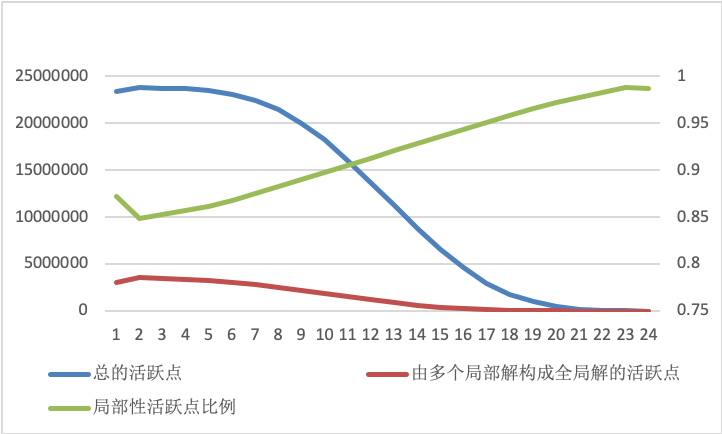
\includegraphics[height=3.8cm,width=0.4\textwidth]{percent-pg-usa.png}}
\hspace{4em}
\bisubcaptionbox{ soc-Live 图上的统计结果\label{fig:percent-pg-soc}
}{Statistical results on the soc-Live graph}
{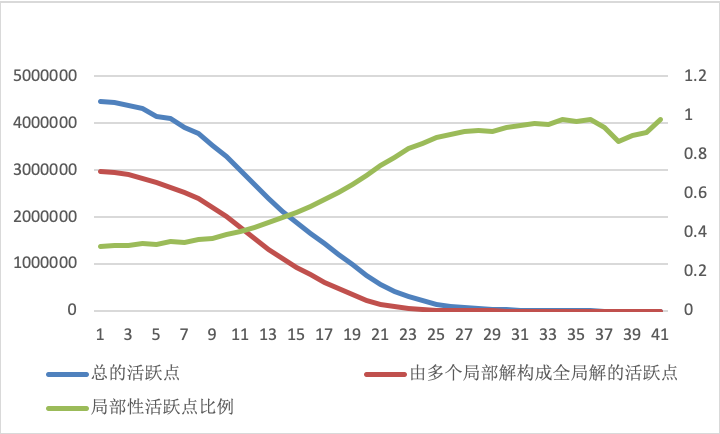
\includegraphics[height=3.8cm,width=0.4\textwidth]{percent-pg-soc.png}}
\hspace{4em}
\bisubcaptionbox{ enwiki 图上的统计结果\label{fig:percent-pg-enwiki}
}{Statistical results on the enwiki graph}
{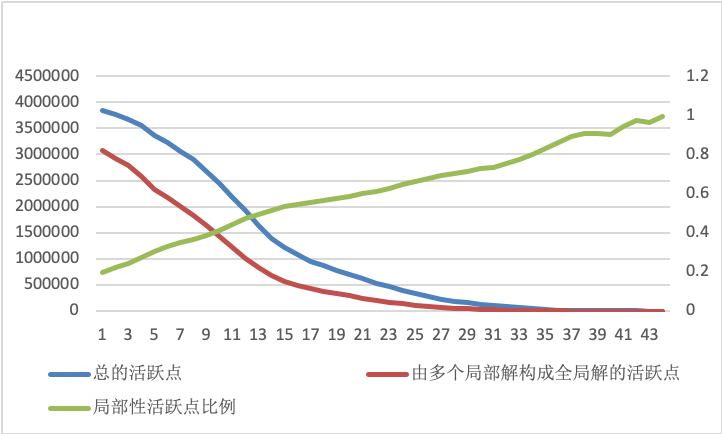
\includegraphics[height=3.8cm,width=0.4\textwidth]{percent-pg-enwiki.png}}
\hspace{4em}
\bisubcaptionbox{ uk-2005 图上的统计结果\label{fig:percent-pg-uk}
}{Statistical results on the uk-2005 graph}
{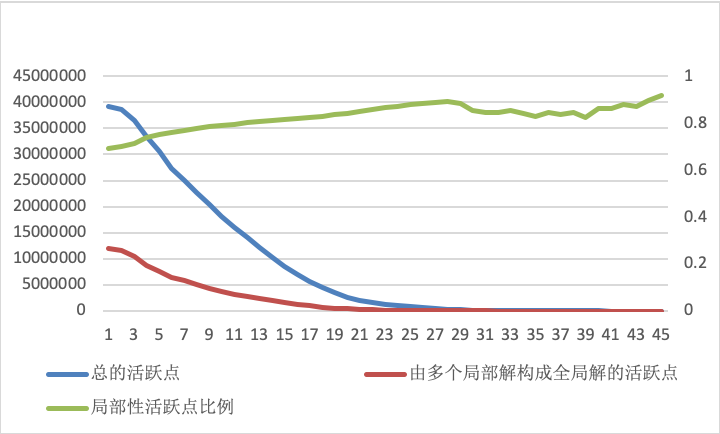
\includegraphics[height=3.8cm,width=0.4\textwidth]{percent-pg-uk.png}}
\hspace{4em}
\bisubcaptionbox{ twitter 图上的统计结果\label{fig:percent-pg-ntw}
}{Statistical results on the twitter graph}
{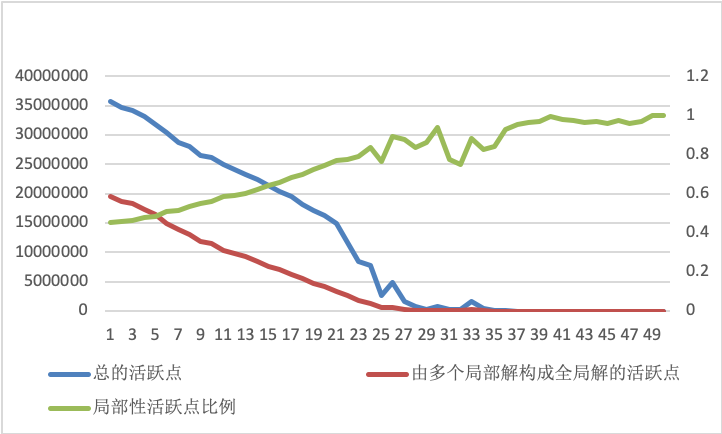
\includegraphics[height=3.8cm,width=0.4\textwidth]{percent-pg-ntw.png}}
\hspace{4em}

  \bicaption{PageRank 算法在不同图上解的局部性的规律统计结果}{Statistical results for the regularity of local solutions of the PageRank algorithm on different graphs.
}
	\label{fig:percent-pg}
\end{figure}



以图\ref{fig:percent-sssp}(\subref{fig:percent-sssp-google})为例,
这个子图给出了SSSP算法在web-Google图上关于解的局部性规律的统计结果。
图中的蓝色曲线给出了图计算迭代过程中总的活跃点的数量先上升后下降的变化趋势。
图中的红色曲线给出了这些活跃点中由多个局部解构成全局解的活跃点的数量变化趋势。
可以看到在整个图计算过程中,这些由多个局部解构成全局解的活跃点都只占总活跃点数量的一小部分。
图中的绿色曲线则具体给出了图计算迭代过程中由单个局部解构成全局解这样具有解的局部性规律的活跃点的比例。
从图中可以看到,在整个图计算过程中,具有解的局部性规律的活跃点的比例始终在94\%以上。
也就是说在图计算过程中,大部分活跃点的全局解都只由单个局部解构成。

图\ref{fig:percent-sssp}(\subref{fig:percent-sssp-youtube}),
\ref{fig:percent-sssp}(\subref{fig:percent-sssp-ca}),
\ref{fig:percent-sssp}(\subref{fig:percent-sssp-usa})给出了
SSSP算法在 com-youtube,roadNet-CA,USA-road图上的统计数据。
这些图上的统计结果也表明了类似的解的局部性规律,尤其是在
roadNet-CA,USA-road这两张图上,
具有解的局部性规律的活跃点的比例一直保持在96\%以上。

图\ref{fig:percent-sssp}(\subref{fig:percent-sssp-soc})给出了
SSSP算法在soc-LiveJournal图上关于解的局部性规律的统计结果。
和前4个图上的统计结果不同,在soc-LiveJournal图上,
由多个局部解构成全局解的活跃点的数量存在一个明显上升然后下降的趋势,
并且上升的数量使得其在总活跃点中占据较高的比例。
相应地,图中表示具有局部性规律活跃点数量比例的绿色曲线呈现出下降后上升的趋势。
在之前的4个图上,绿色曲线虽然也有波动但是一直保持在90\%以上,
而在soc-LiveJournal这个图上,绿色曲线在下降的最低点达到了50\%,随后逐渐上升接近100\%。
也就是说,在迭代的中间阶段,有相当一部分数量的活跃点的全局解由多个局部解构成,
此时解的局部性规律现象不明显,
到了迭代的后期,红色曲线逐渐上升接近100\%,解的局部性规律现象开始出现。
同时对比三条曲线,本研究发现,在活跃点开始下降的时候,具有解的局部性规律的活跃点的比例开始上升。

图\ref{fig:percent-sssp}(\subref{fig:percent-sssp-enwiki}),
\ref{fig:percent-sssp}(\subref{fig:percent-sssp-uk}),
\ref{fig:percent-sssp}(\subref{fig:percent-sssp-ntw})给出了
SSSP算法在 enwiki,uk-2005,twitter图上的统计数据。
在这些图上的统计结果上出现了和soc-LiveJournal图上类似的解的局部性规律。
即在一开始活跃点上升的阶段,由多个局部解构成全局解的活跃点的数量也同样上升,并且占据较高比例,
在活跃点下降之后,由多个局部解构成全局解的活跃点的数量也同样下降,并且占据比例下降。
解的局部性规律在活跃点数量下降的后期才开始出现。



图\ref{fig:percent-cc},\ref{fig:percent-pg}分别给出了 
CC,PageRank 算法在 web-Google, roadNet-CA, com- youtube, USA-road, 
soc-LiveJournal, enwiki, uk-2005, twitter 
这8个大图上关于解的局部性规律的统计结果。
由于是不同的图算法,图中活跃点的变化趋势并不相同。
在SSSP算法中,活跃点是从源点开始一层一层激活的,
在CC算法中,邻居点全都会被激活,
在PageRank算法中,则在一开始就激活全部顶点。
同时由于图算法最终都会收敛,所以活跃点最终都会下降为0。
所以在有些图算法上,活跃点会先上升后下降,在有些图算法上活跃点则会一直下降。

不同的图算法在不同输入图上活跃点的变化趋势虽然不同,
但是在图\ref{fig:percent-sssp},\ref{fig:percent-cc},\ref{fig:percent-pg}这些统计结果上,
解的局部性的规律的却是普遍存在的。
只不过在web- Google,roadNet-CA,com-youtube, USA-road 这些图上,
解的局部性规律一开始就存在,即一开始那些由单个局部解构成全局解的活跃点就一直占据较高的比例,
在soc-LiveJournal,enwiki,uk-2005,twitter 这些图上,
解的局部性规律在一开始不明显,由多个局部解构成全局解的活跃点占据较高比例,
直到活跃点数量开始下降的阶段开始,由单个局部解构成全局解的活跃点才占较高的比例,
解的局部性规律才开始出现。


通过以上分析可以得出这样的结论,
在不同的算法和输入图上都存在着典型的解的局部性规律,
即在每轮的活跃点中,大部分顶点的全局解都只由单个局部解构成,由多个局部解构成全局解的顶点只占极少数,甚至没有。

同时,解的局部性规律虽然普遍存在,但却并不是一开始就存在。
在有些图上,由多个局部解构成全局解的点从一开始就只占极少数,并且数量一直在下降。
而在有些图上,由多个局部解构成全局解的点则存在一个先上升后下降的趋势。
也就是说,解的局部性在有的图和算法的组合上是一直都存在的。
而在另外一些图和算法的组合上,则是随着迭代的进行才逐渐出现。
这也是LazyAsync需要调优才能得到相对最好的性能这一问题的原因。

% 但是在图计算的前期,解的局部性的变化规律则和具体的算法,输入图,以及集群配置有关。

最后,结合图\ref{fig:percent-sssp},\ref{fig:percent-cc},\ref{fig:percent-pg}中的实验结果和之前的决策树策略来分析,
本研究发现决策树中选取的特征和实验结果中揭示的规律是一致的。
决策树策略使用边和顶点的比例$\frac{e}{v}$来表示图的输入图本地性,
针对那些 $\frac{e}{v} \textless 10$  的图,系统直接开启LazyAsync,就能获得相对较好的性能提升。
而在本研究的实验中发现,在 $\frac{e}{v} \textless 10$ 的web-Google,roadNet-CA,com-youtube,
USA-road 这4个图上,确实一开始就存在着解的局部性的规律。
针对那些 $\frac{e}{v} \textgreater 10$ 的图, 决策树指导系统在活跃点下降率超过7\%时开启LazyAsync,然后就能获得相对较好的性能提升。
而在本研究的实验中发现,在$\frac{e}{v} \textgreater 10$的 soc-LiveJournal,enwiki,uk-2005,twitter 这4个图上,
活跃点下降超过7\%的时间节点,也是由多个局部解构成全局解的活跃点数量开始下降,解的局部性的规律开始出现的时候。

% 同时对于决策树失灵的情况
%结果分析

\section{基于解的局部性的自适应优化方法}


\algnewcommand{\LeftComment}[1]{\Statex \(\triangleright\) #1}

\begin{algorithm}[!htbp]
  \small
  \caption{消息交换中在线统计全局解和局部解关系的算法}\label{alg:exchange_msg}
  \begin{algorithmic}[1] 
      \Require $G(V, E, D)$
      \Require multiLocal:\quad vertex set that contains multiple local soultion 
      \Procedure{ExchangeDeltaMsg}{}
      \LeftComment{Stage1: msg exchange : mirror send deltamsg to  master }

      \For{ \textbf{parallel} v $: has\_message\_global$ }
      \If{ v is mirror }
      \State send deltamsg to master
      \Else{}
      \State append deltamsg to $messages\_global\_sum$
      \State set $has\_message\_global\_sum$

      {\color{red}
      \If{ v in $has\_message\_global\_sum$ }
      \State set multiLocal[v]
      \EndIf
      }

      \EndIf
      \EndFor

      \For{ \textbf{parallel} v $: recv\_buffer$ }
      \State ASSERT\_TRUE(v is master)
      \State append deltamsg to $messages\_global\_sum$
      \State set $has\_message\_global\_sum$
      {\color{red}
      \If{ v in $has\_message\_global\_sum$ }
      \State set multiLocal[v]
      \EndIf
      }
      \EndFor

      \LeftComment{Stage2: msg exchange : master send sum to  mirrors }

      \For{ \textbf{parallel} v $: has\_message\_global\_sum$ }
      \If{ v is master }
      \State send global\_sum to mirrors
      \State set messages \& $has\_message$
      \EndIf
      \EndFor

      \For{ \textbf{parallel} v $: recv\_buffer$ }
      \State set messages \& $has\_message$
      \EndFor
      \EndProcedure
    \end{algorithmic}
\end{algorithm}


\begin{algorithm}[!htbp]
  \small
  \caption{基于解的局部性的自适应优化算法}\label{alg:adaptive}
  \begin{algorithmic}[1] 
      \Require $G(V, E, D)$
      \Require activeCurr:\quad Initial active vertex set activeCurr
      \Require multiLocal:\quad vertex set that contains multiple local soultion 

      % \Ensure output
      \While{$iteration \leq maxIteration$}
      \LeftComment{Stage1: local computation stage}
      \If{$enableLazy \  is \  true$} 
      \For{\textbf{parallel} $activeCurr$}
      \If{$activeCurr \  is \  NULL$ \textbf{or} $doLC() \  is \  false$}
      \State $break$
      \EndIf
      \State $Applys()$
      \State $ScatterGatherMsgs()$
      \State $activeCurr = activeNext$;\quad $activeNext = NULL$
      \EndFor
      \EndIf

      \State $enableLazy = false$

      \State $ExchangeDeltaMsgs()//$详见算法\ref{alg:exchange_msg}
      \State multiLocalCurr = rmi.all\_reduce(multiLocal)
      \State $barrier()$
      \If{$msgEmpty() \  \textbf{and} \  activeEmpty()$}
      \State $break$
      \EndIf
      {
      \color{red}
      \If{ $\frac{e}{v} \textless 10 \quad ||  \quad   multiLocalCurr \textless multiLocalLast $ }
      \State $enableLazy = true$
      \EndIf
      }
      
      \LeftComment{Stage2: data coherency stage}

      \For{\textbf{parallel} $activeCurr$}
      \State $Applys()$
      \State $ScattersGatherMsgs()$
      \State $activeCurr = NULL$
      \EndFor

      \State multiLocalLast = multiLocalCurr
      \State $activeCurr = activeNext$;\quad $activeNext = NULL$; \quad $iteration ++$
      \EndWhile
  \end{algorithmic}
\end{algorithm}

在上一节中,本研究通过实验证明了在图计算过程中确实存在着解的局部性规律。
解的局部性这种规律和具体的输入图及算法有关,在迭代的某个时间节点之后才存在。
通过统计全局解由多个局部解构成的顶点的数量,本研究可以观察和判断出解的局部性。


LazyAsync的性能提升受冗余计算的影响。而解的局部性则可以用于减少冗余计算。
基于此,本研究最终提出了一种基于解的局部性的自适应优化方法,它指导LazyAsync
在图计算开始出现的解的局部性的时候来开启 lazy data coherency 。

在之前的实验中,本研究通过保存局部解的方式在图计算完成之后对迭代过程中解的局部性进行观察。
这种事后离线实验的方式只能用于观察图计算过程中的规律,却无法直接作为开启策略。
为了实现基于解的局部性的自适应优化方法,本研究需要找到一种在线的统计方式。

在之前的实验中,为了观察局部解的具体数量和数值,本地累加和需要被记录保存。
但是如果只是为了统计全局解由多个局部解构成的顶点的数量,本地累加和并不需要被记录保存。
分析消息交换的过程可以发现,只需要在消息交换的过程增加一些判断条件,
本研究就能实现在线地统计全局解由多个局部解构成的顶点的数量这一目的。
算法\ref{alg:exchange_msg}给出了本研究在消息交换中在线统计全局解和局部解关系这一算法的伪代码,
其中红色部分标出了本研究在消息交换过程中添加的判断条件。

如算法\ref{alg:exchange_msg}所示,在消息交换的第一个阶段,标记为mirror的副本点向标记为master的副本点
发送消息。这份消息中包含本地子图的消息累加和,构成了局部解。
同时对于标记为master的副本点而言只需要在本地直接把消息添加到内存的数组中。
对于一个顶点而言,它的全局解由来自master和多个mirror的局部解共同构成。
通过在消息交换第一阶段master顶点接收局部解时判断mater点上是否已经有局部解,本研究就能知道
该顶点的全局解是由多个局部解构成还是由单个局部解构成。
当顶点的全局解由单个局部解构成时,这个局部解既可能来自master也可能来自某个mirror。
当顶点的全局解由多个局部解构成时,这些局部解可能只来自部分副本点,因为有些副本点上很有可能未被激活没有局部解。
此外考虑到分布式系统中的消息时延和并发处理的不确定性,本研究无法确定来自其他副本的消息和本地master的消息谁更早被写入到内存数组中。

综合考虑以上这些条件,本研究在master写本地消息的地方(即算法\ref{alg:exchange_msg} line 8)
和接收远程消息的地方(即算法\ref{alg:exchange_msg} line 17)分别加了判断条件,如果写消息时或收消息时顶点上已经有局部解了,
那么这个顶点上的全局解就由多个局部解构成,相应地要将 multiLocal 这个 bitset 进行标记置位。
在消息发送的第一阶段,本地写消息和接收远程消息都只发生在标记为master的副本点上,对全局解和局部解关系的判断也只发生在标记为master的副本点上。
在消息交换整个阶段完成之后,各个活跃点的副本点都得到了相同的消息累加和,同时那些由多个局部解构成全局解的顶点也已经被标记置位。
此时,通过mpi提供的all\_reduce操作对集群中各个结点的进程实例中的multiLocal进行规约求和,
本研究就基于在线统计的方法得到了上一轮迭代中由多个局部解构成全局解的顶点的数量。
相较于4.3节中采用的离线统计方法,这种方法不需要在顶点上额外保存变量,也不需要导出文件,不影响计算过程,
只需要在消息交换中添加if判断条件并进行一个mpi提供的all\_reduce规约操作,开销很小。



实现了在线即时统计全局解由多个局部解构成的顶点的数量这一目的之后,
本研究就真正的得到了一个基于解的局部性的自适应优化方法。
这个基于解的局部性的自适应优化方法由算法\ref{alg:exchange_msg}和算法\ref{alg:adaptive}共同构成。
在算法\ref{alg:exchange_msg}的基础上,算法\ref{alg:adaptive}给出了系统如何根据
图的本地性($\frac{e}{v}$)和全局解由多个局部解构成的顶点的数量这两个指标自适应地判断是否启用LazyAsync这一过程的伪代码。
不同的输入图其边点数量比$\frac{e}{v}$各不相同,所以图的本地性这个指标反映了对输入图的自适应。
集群环境和划分算法以及算法用例则会对副本点和副本点上的局部解产生影响,
所以全局解由多个局部解构成的顶点的数量变化趋势这个指标反映了对运行环境变化的自适应。

在算法\ref{alg:adaptive}中可以看到,基于解的局部性的自适应优化方法的关键代码其实就是对两个指标的进行的if判断。
但是这个判断正是对4.2节实验中发现的解的局部性变化规律的应用。
在4.2节本研究通过实验发现,那些本地性指标$\frac{e}{v} \textless 10$ 的图在各种算法上在迭代一开始就一直表现出明显的解的局部性现象,
所以在自适应优化方法中判断立即启用LazyAsync。
对那些本地性指标$\frac{e}{v} \textgreater 10$ 的图,通过实验发现,在全局解由多个局部解构成的顶点的数量开始下降时,
由单个局部解构成全局解这样具有解的局部性规律的活跃点的比例开始上升并趋近100\%。
所以在自适应优化方法中本研究在观察到$  multiLocalCurr \textless multiLocalLast$ 这一条件时才启用LazyAsync。


\section{性能评测}

在本节中,本研究在48台虚拟机构成的集群环境中,对比了PowerGraph原始的同步引擎,
LazyGraph的手动调优方法和LazyGraph的自适应优化方法
这三种方式下的性能。

\subsection{实验环境}
\begin{table}[htb]
  \centering
  \bicaption{实验平台}{Experimental Methodology}
  \label{tab:experimental_methodology}
    \begin{tabular}{cccccc}
     \toprule[1.5pt]
     \multicolumn{5}{c}{\textbf{Each Node}} &   \multirow{2}{*}{\textbf{Cluster}} \\
     \cmidrule(lr){1-5}
     Compiler & CPU & Memory & System & Network \\
     \midrule[1pt]
     GCC 4.4.7 & 8 Intel Xeon cores & 32GB & CentOS 6.5  & 1 GigE Ethernet & 48-node cluster\\
     \bottomrule[1.5pt]
    \end{tabular}
\end{table}



\begin{table}[htb]
  \centering
  \bicaption{实验数据集及划分算法}{Experimental Data Set and Partition Algorithm}
  \label{tab:experimental_data_set_and_partition_algorithm}
    \begin{tabular}{ccccccc}
     \toprule[1.5pt]
     & \textbf{Graph} & \textbf{\#V} & \textbf{\#E} & \textbf{E/V} & \textbf{$\lambda$} & {\textbf{Partition Algorithm}} \\
     \midrule[1pt]
     \multirow{2}{*}{web} & UK-2005 & 40M & 936M & 23.73 & 3.51 & \multirow{8}{*}{Coordinated Vertex-Cut } \\
                                         & web-Google & 0.9M & 5.1M & 5.83 & 2.47 \\
     \cmidrule(lr){1-6}
      \multirow{2}{*}{road} & road-USA-net & 24M & 58M & 2.44 & 2.14 \\
                                          & roadNet-CA & 2M & 5.5M & 2.82 & 2.09 \\
      \cmidrule(lr){1-6}
      \multirow{4}{*}{social} & twitter & 61.58M & 1468M & 23.85 & 5.52 \\
                                          & soc-LiveJournal & 4.84M & 68.9M & 14.23 & 4.96 \\
                                          & enwiki & 4.2M & 101.36M & 24.09M & 7.22 \\
                                          & com-youtube & 1.1M & 6M & 5.27M & 2.70 \\
     \bottomrule[1.5pt]
    \end{tabular}
\end{table}

为了评测本研究所提出的自适应优化方法的效果,本研究在由48台虚拟机构成的集群环境中测试了
PowerGraph的原始同步引擎,LazyGraph的手动调优方法,和基于解的局部性的自适应优化方法
这三种方式下的性能结果。
如表\ref{tab:experimental_methodology}所示,每个节点上的操作系统是Centos 6.5,
配置的编译器版本为4.4.7,配置的CPU有8个核,内存有32GB,
集群的节点之间以1GigE的以太网连接。
实验过程中使用的数据集总共包含3个类型,8个不同大小的真实图。
这些数据集同4.2节中使用的一样,具体元数据如表\ref{tab:experimental_data_set_and_partition_algorithm}所示。
同时,本研究均使用 coordinated vertex-cut 划分算法来做图的划分。
实验过程中使用了
SSSP, 
Connected Component(CC),
K-core Decomposition(kcore), 
Page Rank这四种典型的图算法来作为测试用例。


\subsection{实验结果}

\begin{figure}[h]
	\centering
  \captionsetup{justification=centering}
	\bisubcaptionbox{ SSSP 的加速比\label{fig:speedup_sssp}}{Speedup in SSSP}
	%[3cm] %标题的长度,超过则会换行,如下一个小图。
	{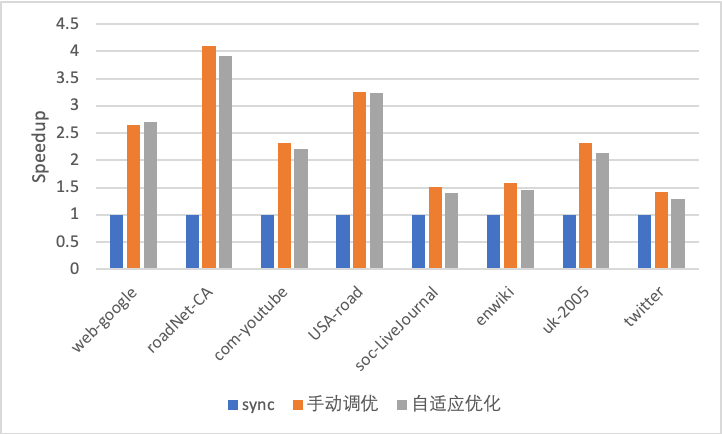
\includegraphics[height=4.5cm,width=0.4\textwidth]{speedup_sssp.png}}
  \hspace{4em}% 这里记得不要空行,否则会变为垂直的两个图
	\bisubcaptionbox{CC 的加速比\label{fig:speedup_cc}}{Speedup in CC}
	%[3cm] %标题的长度,超过则会换行,如下一个小图。
	{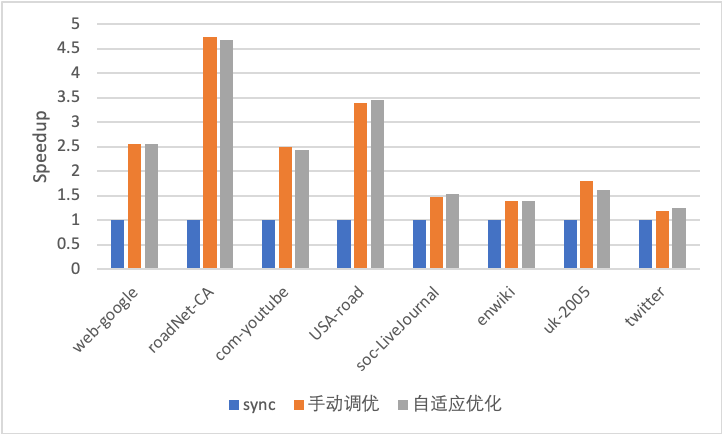
\includegraphics[height=4.5cm,width=0.4\textwidth]{speedup_cc.png}}
	\hspace{4em}% 这里记得不要空行,否则会变为垂直的两个图
	\bisubcaptionbox{K-Core 的加速比\label{fig:speedup_kcore}}{Speedup in K-Core}
	%[3cm] %标题的长度,超过则会换行,如下一个小图。
	{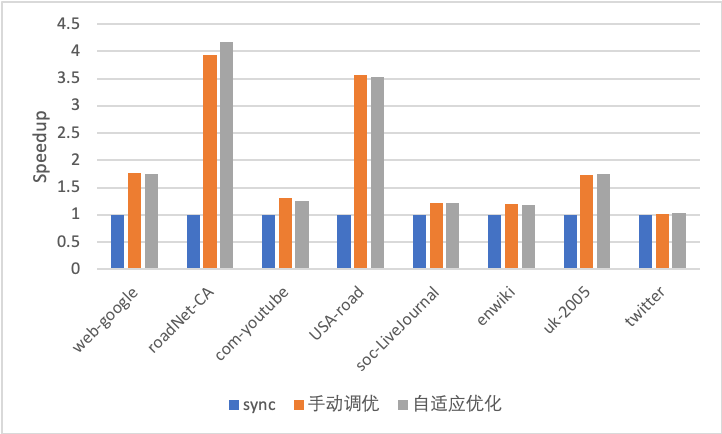
\includegraphics[height=4.5cm,width=0.4\textwidth]{speedup_kcore.png}}
	\hspace{4em}% 这里记得不要空行,否则会变为垂直的两个图
	\bisubcaptionbox{PageRank 的加速比\label{fig:speedup_pagerank}}{Speedup in PageRank}
	{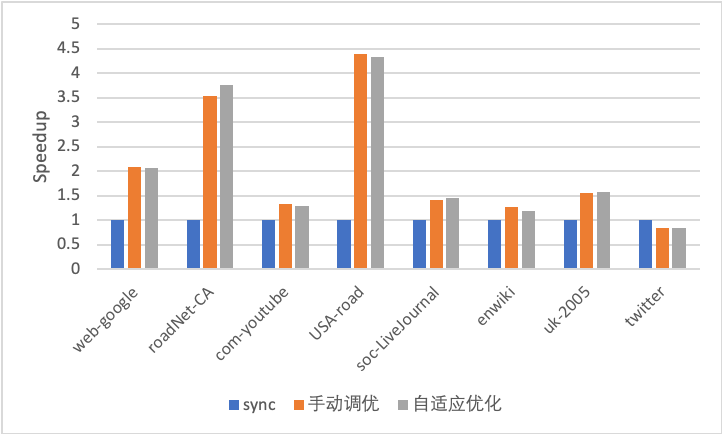
\includegraphics[height=4.5cm,width=0.4\textwidth]{speedup_pagerank.png}}
	\bicaption{ SSSP,CC,K-Core和PageRank 在48机真实图上的性能对比}{Speedup Comparisons for SSSP, CC ,K-Core and  PageRank on Real-World Graphs on 48 Machines}
	\label{fig:speedup_four_algorithm}
\end{figure}


\begin{figure}[h]
  \centering
  \captionsetup{justification=centering}
  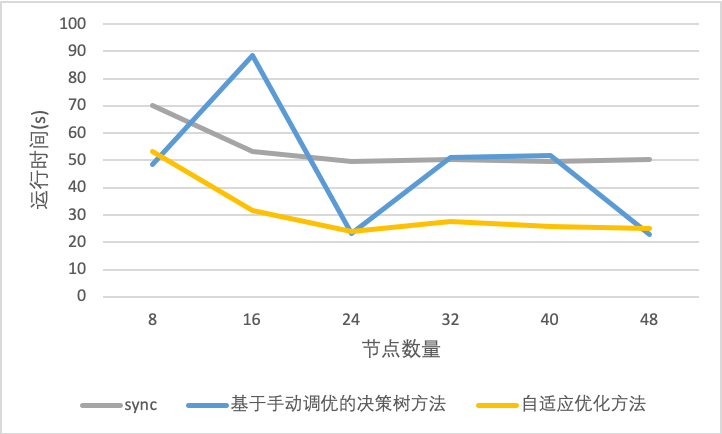
\includegraphics[width=0.8\textwidth]{sssp-uk-dt-vs-opt}
  \bicaption{不同集群配置下,SSSP 算法在 uk-2005输入图上的运行时间}{Runtime of the SSP algorithm on the uk-2005 input graph with different cluster configurations}
  \label{fig:dt-vs-opt}
\end{figure}

图 \ref{fig:speedup_four_algorithm} 展示了四种图算法在8个不同的输入图上分别采用
PowerGraph 原始同步引擎,
LazyGraph 手动调优方法,
LazyGraph 基于解的局部性的自适应优化方法
这三种方式进行计算所得到的性能测试结果。
可以看到,
在不同的算法和输入图的组合上,LazyGraph的表现性能都好于PowerGraph。
而在LazyGraph 上, 基于解的局部性的自适应优化方法
得到的性能提升效果
和手动调优方式下得到的相当,甚至有时超过了后者。

在手动调优的方法中,我们通过不断的尝试分别在不同的迭代轮次开启LazyAsync然后取其中最好的值作为最终结果。
在自适应优化方法中,本研究通过在线地观察解的局部性方式来自动选择LazyAsync的开启轮次。
通过对比,本研究发现,自适应优化方法所自动选择的开启轮次和手动调优方法中最后结果对应的开启轮次是基本一致的。
这也正是自适应优化方法能够得到和手动调优方法效果相一致甚至超过后者的原因。



图\ref{fig:dt-vs-opt}则给出了在不同的集群配置下,SSSP 算法在 uk-2005这个输入图上分别采用原始同步引擎,
基于手动调优得到的决策树方法,基于解的局部性的自适应优化方法 这三种方法所用的运行时间。
从图中可以看到,从8台机器到48台机器,基于解的局部性的自适应优化方法保持了较好的可扩展性,运行时间先下降然后稳定。
而基于手动调优得到的决策树方法则出现了不正常的数据波动,在16,32,40台机器时性能没有得到提升甚至下降。
这也正是前文研究动机中提到的决策树失灵的情况。

我们通过在手动调优得到的最佳组合进行数据拟合得到了决策树方法。
这种方法在局部性不好的图上观察到包含所有副本在内的活跃点数量下降超过一定比例时开启LazyAsync。
在局部性不好的图上,活跃点下降时往往也是解的局部性规律开始出现的时候,所以在一些情况下,
决策树方法也能得到和手动调优相一致的效果。
但是,集群的配置会影响图划分,图划分影响顶点的副本点个数,最终集群配置变化会导致活跃点数量的变化。
在决策树失灵所对应的这些集群配置中,活跃点数量的变化导致决策树误判提前开启了LazyAsync
而此时解的局部性现象还没有出现,提前开启就会在本地计算中引入大量的冗余计算,
最终使得性能没有得到提升甚至下降。

  
通过以上比较可以得出结论,
基于解的局部性的自适应优化方法确实能够替代繁琐的手动调优方法,自动地得到相对最优的性能提升效果。
同时这种方法也能正确处理基于手动调优得到的决策树方法失灵的情况。


\section{本章小结}
在本章中,本研究先是通过小例子直观说明了全局解和局部解的关系如何影响LazyAsync中存在的冗余计算。
在此基础上,本研究提出了解的局部性的概念。
当顶点上的全局解只由某一个局部解构成时,在顶点上开启LazyAsync能够避免冗余计算。
当大部分顶点上的全局解都只由某个局部解构成时,本研究称之为解的局部性。
解的局部性现象有利于开启LazyAsync。

本研究在不同算法和输入图的组合的迭代过程中解的局部性规律进行了统计。
统计结果表明在各种算法和输入图的组合中,解的局部性规律是普遍存在的。
不过在有些组合上,这种规律一开始就一直存在,在其他组合上,这种规律在迭代进行一段时间后才存在。

基于解的局部性这一规律,本研究最终实现了一种在线的自适应优化方法。
这种方法在线地统计活跃点中由单个局部解构成全局解的顶点的数量和比例,
当这样的顶点占多数时就开启LazyAsync,当这样的点占少数时就关闭LazyAsync。
在4种常见经典图算法和8个大图数据集上的实验结果表明,这种方法取得了和手动调优方法相一致的性能提升效果。
